\documentclass[../../main.tex]{subfiles}
\usepackage{amsmath}	% required for `\align' (yatex added)
\usepackage{pgfplots}
\pgfplotsset{compat=1.18}
\begin{document}

{\bf[解]}
簡単のため$c = \cos\theta, s = \sin\theta$ とおく ($0 \le \theta < 2\pi$)と，
題意から$(x,y)$は半径$1$の円周上にあるから $(x,y) = (c,s)$ とおける．

$f(\theta) = c^2 - s^2 + 2\sqrt{3}cs$ とすると倍角公式および三角関数の合成より
\begin{align}
  f(\theta) 
 & = \cos 2\theta + \sqrt{3}\sin 2\theta \\
 &= 2\sin\left(2\theta + \dfrac{\pi}{6}\right) 
\end{align}
と書ける．$0 \le \theta < 2\pi$にも注意すると，
$f(\theta)$ が最大の時，$\theta = \dfrac{\pi}{6}, \dfrac{7}{6}\pi$ で $(x,y) = \left(\dfrac{\sqrt{3}}{2}, \dfrac{1}{2}\right), \left(-\dfrac{\sqrt{3}}{2}, -\dfrac{1}{2}\right)$である．

$f(\theta)$ が最小の時，$\theta = \dfrac{2}{3}\pi, \dfrac{5}{3}\pi$ で $(x,y) = \left(-\dfrac{1}{2}, \dfrac{\sqrt{3}}{2}\right), \left(\dfrac{1}{2}, -\dfrac{\sqrt{3}}{2}\right)$．
である．以上まとめると
\begin{align}
 (x,y) = 
 \begin{cases}
  \left(\dfrac{\sqrt{3}}{2}, \dfrac{1}{2}\right), \left(-\dfrac{\sqrt{3}}{2}, -\dfrac{1}{2}\right) & (\text{最大}) \\
  \left(-\dfrac{1}{2}, \dfrac{\sqrt{3}}{2}\right), \left(\dfrac{1}{2}, -\dfrac{\sqrt{3}}{2}\right) & (\text{最小})  
 \end{cases}
\end{align}
が求める$(x,y)$の値である．

{\bf [解説]}

単なる三角関数の最大最小問題に落とし込める．今回の$f(\theta)$の概形は以下のようになる．
\begin{figure}[htb]
\begin{center}
 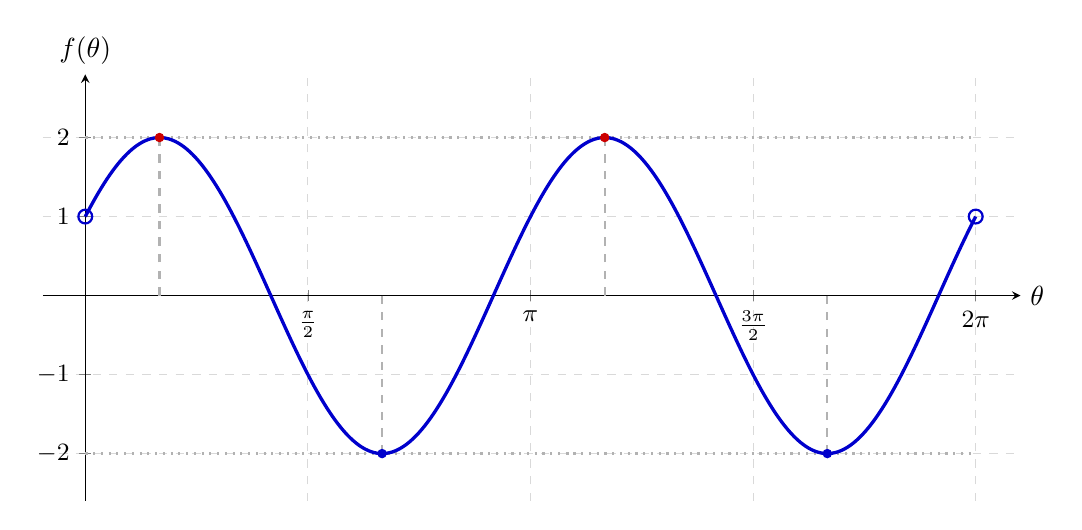
\begin{tikzpicture}
\begin{axis}[
    % 軸の設定
    axis lines = middle,
    xlabel = {$\theta$},
    ylabel = {$f(\theta)$},
    trig format plots = rad,   
    % 表示範囲
    xmin = -0.3, xmax = 6.6,
    ymin = -2.6, ymax = 2.8,
    % 目盛りの位置 (pi/2 刻み)
    xtick = {1.5708, 3.1416, 4.7124, 6.2832},
    xticklabels = {$\frac{\pi}{2}$, $\pi$, $\frac{3\pi}{2}$, $2\pi$},
    ytick = {-2, -1, 1, 2},
    % グリッド線
    grid = major,
    grid style = {dashed, gray!30},
    % ラベル位置の調整
    xlabel style = {at={(ticklabel* cs:1)}, anchor=west},
    ylabel style = {at={(ticklabel* cs:1)}, anchor=south},
    ticklabel style = {font=\small},
    % アスペクト比の設定
    width = 14cm,
    height = 7cm
]

    % y = 2, y = -2 の振幅補助線
    \addplot[thick, dotted, gray!60, domain=0:2*pi] {2};
    \addplot[thick, dotted, gray!60, domain=0:2*pi] {-2};

    % メイングラフ (0 < theta < 2pi)
    \addplot [
        domain = 0:2*pi,
        samples = 300,
        color = blue!80!black,
        very thick
    ]
    {2*sin(2*x + pi/6)};

    % theta = 0 での端点（白抜き丸）
    \addplot[only marks, mark=o, mark size=2.5pt, thick, color=blue!80!black] coordinates {(0, 1)};
    \node[left, font=\small] at (axis cs:0, 1) {};

    % theta = 2pi での端点（白抜き丸）
    \addplot[only marks, mark=o, mark size=2.5pt, thick, color=blue!80!black] coordinates {({2*pi}, 1)};

    % 山の頂点（最大値 2）
    \pgfplotsinvokeforeach{0.5236, 3.6652}{
        \addplot[only marks, mark=*, mark size=1.5pt, color=red!80!black] coordinates {(#1, 2)};
        \draw[gray!60, dashed, thick] (axis cs:#1, 0) -- (axis cs:#1, 2);
    }
    % 谷の底（最小値 -2）
    \pgfplotsinvokeforeach{2.0944, 5.2360}{
        \addplot[only marks, mark=*, mark size=1.5pt, color=blue!80!black] coordinates {(#1, -2)};
        \draw[gray!60, dashed, thick] (axis cs:#1, 0) -- (axis cs:#1, -2);
    }

\end{axis}
\end{tikzpicture}
\caption{$f(\theta)$の概形とその最大最小値．}
\end{center}
\end{figure}


\newpage

\end{document}
